\documentclass[11pt]{article}
\usepackage[review]{acl}
\usepackage{times}
\usepackage{latexsym}
\usepackage[T1]{fontenc}
\usepackage[utf8]{inputenc}
\usepackage{microtype}
\usepackage{inconsolata}
\usepackage{graphicx}
\usepackage{booktabs}
\usepackage{amsmath}
\usepackage{amssymb}
\usepackage{multirow}
\usepackage{array}
\usepackage{url}

\newcommand{\ApiTotal}{1,388,276}
\newcommand{\AttrDec}{100.0\%}
\newcommand{\AttrUnres}{0.0\%}
\newcommand{\BestCtx}{SENT}
\newcommand{\BestF}{0.891}
\newcommand{\BestModel}{distilroberta-base}
\newcommand{\ChainIssueSpecific}{42.7\%}
\newcommand{\CourtHi}{1 Cir.}
\newcommand{\CourtHiRate}{26.99\%}
\newcommand{\CourtLo}{4 Cir.}
\newcommand{\CourtLoRate}{12.27\%}
\newcommand{\CtxWorstDelta}{-0.300}
\newcommand{\CtxWorstHi}{-0.167}
\newcommand{\CtxWorstLo}{-0.421}
\newcommand{\DictSHA}{c23210667a4e}
\newcommand{\EscCIHi}{-5.4}
\newcommand{\EscCILo}{-10.0}
\newcommand{\EscDec}{100.0\%}
\newcommand{\EscDiffPP}{-7.5}
\newcommand{\EscNotOpen}{99.1\%}
\newcommand{\EscOpen}{91.6\%}
\newcommand{\EscUnres}{50.0\%}
\newcommand{\ExtractYield}{61.9\%}
\newcommand{\HOneUnresShare}{85\%}
\newcommand{\HeldOutCourts}{5 Cir., D.C. Cir.}
\newcommand{\HumanAgree}{90.3\%}
\newcommand{\HumanFlip}{9.7\%}
\newcommand{\HumanUnclearFull}{12.9\%}
\newcommand{\HumanUnclearSent}{22.6\%}
\newcommand{\IMEscRate}{40\%}
\newcommand{\IndepDec}{0.0\%}
\newcommand{\IndepUnres}{50.0\%}
\newcommand{\IssueOnlyAcc}{60.6\%}
\newcommand{\IssueOnlyF}{0.541}
\newcommand{\JudgeLexF}{0.567}
\newcommand{\JudgeTfidfF}{0.481}
\newcommand{\LCCross}{80}
\newcommand{\LCTopAcc}{0.947}
\newcommand{\LLMBestCtx}{W256}
\newcommand{\LLMBestF}{0.774}
\newcommand{\LLMDevice}{Tesla T4}
\newcommand{\LLMDtype}{float16}
\newcommand{\LLMMinutes}{12.1}
\newcommand{\LLMName}{Phi-3.5-mini-instruct}
\newcommand{\LLMRevision}{2fe192450127}
\newcommand{\LLMSentF}{0.742}
\newcommand{\LLMWideF}{0.437}
\newcommand{\LexF}{0.946}
\newcommand{\LexHOne}{0.895}
\newcommand{\MedWords}{1,921}
\newcommand{\NAnnotated}{364}
\newcommand{\NBench}{306}
\newcommand{\NCandRaw}{289,206}
\newcommand{\NChainOrigins}{177}
\newcommand{\NChainPassages}{3,347}
\newcommand{\NChains}{3,347}
\newcommand{\NCharLZero}{1,077}
\newcommand{\NCharLoose}{4,863,357}
\newcommand{\NCharOps}{22,471}
\newcommand{\NCharTight}{79,974}
\newcommand{\NDec}{3}
\newcommand{\NDev}{120}
\newcommand{\NDrawn}{1,800}
\newcommand{\NEligible}{928,254}
\newcommand{\NEscN}{58,600}
\newcommand{\NEscOps}{18,506}
\newcommand{\NFedApp}{1,998,580}
\newcommand{\NFrameCtrl}{169,952}
\newcommand{\NFrameTrigger}{179,160}
\newcommand{\NHumanAbl}{31}
\newcommand{\NIMDistinct}{10}
\newcommand{\NIMEsc}{4}
\newcommand{\NIMGenuine}{15}
\newcommand{\NIMMatched}{27}
\newcommand{\NIMPrec}{56\%}
\newcommand{\NIssueSpecific}{1,428}
\newcommand{\NJudgeBench}{2,252}
\newcommand{\NJudgeDec}{1,899}
\newcommand{\NJudgeUnres}{353}
\newcommand{\NLayerTwo}{23}
\newcommand{\NLayerTwoAnnotated}{23}
\newcommand{\NLayerTwoUsable}{5}
\newcommand{\NOccurrences}{250,781}
\newcommand{\NProxyCheck}{17}
\newcommand{\NProxyGood}{2}
\newcommand{\NScanned}{10,798,347}
\newcommand{\NTextFields}{4}
\newcommand{\NUnclear}{58}
\newcommand{\NUnres}{2}
\newcommand{\NWithTrigger}{175,610}
\newcommand{\NWordsBn}{2.67}
\newcommand{\OCRShare}{22.5\%}
\newcommand{\OffIssueRate}{78\%}
\newcommand{\PassMinutes}{114}
\newcommand{\PeriodFirstRate}{15.88\%}
\newcommand{\PeriodLastRate}{22.36\%}
\newcommand{\PeriodRatio}{1.4}
\newcommand{\PrevMajority}{19.59\%}
\newcommand{\PrevPub}{20.85\%}
\newcommand{\PrevSeparate}{9.93\%}
\newcommand{\PrevUnpub}{9.21\%}
\newcommand{\Prevalence}{18.92\%}
\newcommand{\ProxyPrec}{12\%}
\newcommand{\RecallHit}{17.8\%}
\newcommand{\RecallSampled}{4,000}
\newcommand{\ShareAssumed}{12.6\%}
\newcommand{\ShareAvoided}{86.9\%}
\newcommand{\ShareIssueSpecific}{42.7\%}
\newcommand{\ShareReserved}{0.5\%}
\newcommand{\ShareUnresolved}{65.0\%}
\newcommand{\ShareWhether}{66.4\%}
\newcommand{\TemporalCut}{2018}
\newcommand{\TfidfBestF}{0.813}
\newcommand{\YearMax}{2026}
\newcommand{\YearMin}{1789}


\title{Need Not Decide: A Benchmark for Judicial Non-Resolution\\
in U.S. Federal Appellate Opinions}

\author{Author Name \\
  Affiliation \\
  \texttt{email@domain}}

% Subsection headings replace the run-in bold paragraph headings; the default
% vertical space around them is generous for a two-column layout, so it is
% tightened rather than dropping content to stay inside the page limit.
\usepackage{capt-of}
% Allow more than one full-width float at the top of a page, so the
% supplementary tables do not flush onto a page of their own.
\setcounter{dbltopnumber}{4}
\renewcommand{\dbltopfraction}{.92}
\renewcommand{\dblfloatpagefraction}{.7}
\setcounter{topnumber}{3}
\renewcommand{\topfraction}{.9}
\renewcommand{\textfraction}{.06}
\usepackage{titlesec}
\titlespacing*{\subsection}{0pt}{4pt plus 1pt minus 1pt}{1pt}
\titleformat{\subsection}{\normalfont\bfseries}{\thesubsection}{0.6em}{}

\begin{document}
\maketitle

\begin{abstract}
Deciding less than it could is one of the ways an appellate court exercises
authority, and courts announce it in a small vocabulary that has been stable for
a century. We ask whether language models can tell an issue a court resolved
from one it discussed and left open, and what becomes of an unresolved issue as
later courts cite it. A frozen
thirteen-expression dictionary applied to \NEligible{} federal appellate
opinions from the CourtListener bulk release finds explicit non-resolution
language in
\Prevalence{}. From that population we draw a stratified benchmark of \NBench{}
annotated issues, pairing trigger-bearing passages with matched issues from
trigger-free opinions and with two adversarial strata where the trigger is
present but misleading. The dictionary scores well pooled, but that score is an
artefact of anchor-centred sampling. Per
stratum the systems separate: supervised models beat the dictionary on the
stratum built to defeat it, and a fine-tuned encoder beats it outright on the
court-held-out condition. Context helps to about $\pm256$ characters and then
hurts. We release \NCharTight{} judicially authored characterizations of prior
decisions and use them to hand-verify cases
where a later court calls a declined question a holding, which bears on how
citation counts are read as evidence of what an opinion settled. The dictionary,
benchmark, and pipeline are released.
\end{abstract}

\section{Introduction}

Courts are unusual among institutions in that their output is a written account
of their own reasoning, so what they decline to do is recorded in the same
medium as what they do. A United States appellate court that has raised a legal
question is not obliged to answer it. It may resolve the case on a narrower ground and say that it
``need not decide'' the question. It may assume an answer ``without deciding''
and show that the outcome is the same either way. It may state that the question
is left ``for another day.'' These moves are ordinary, and they are marked in
prose by a small vocabulary that has been stable for a century.

Declining to decide is a choice about how much law to make. It is the working
form of the norm that a court should rule no more broadly than the case
requires, and it is one of the few exercises of judicial discretion that leaves
a direct textual trace instead of having to be inferred from votes or outcomes.

The practice matters for two reasons that pull in different directions. For
courts, declining to decide is a discipline, the means by which a court keeps its
holdings narrow and leaves a question open for a better-argued case. For anyone
who later reads the opinion, it is a trap. An opinion that assumed a proposition
without deciding it reads, at the level of the sentence, like an
opinion that held it. The distinction lives in the surrounding paragraphs, and
sometimes in a footnote several pages away.

That combination makes judicial issue disposition a natural test for language
technology. The label depends on discourse structure rather than lexical content,
the surface cue is easy to find and easy to misread, and there is an external
record of what happened next. This paper builds a task around it and uses the
task to ask an institutional question.

\subsection{Two layers} We separate a classification problem from the phenomenon
it lets us study. For an issue $q$ appearing in opinion $o$, layer one asks for
\begin{equation}
D(q,o) \in \{\textsc{decided}, \textsc{unresolved}\},
\end{equation}
with \textsc{unresolved} refined into \textsc{avoided}, \textsc{assumed}, and
\textsc{reserved}. The primary benchmark is deliberately binary. Layer two takes
an issue $q$ that opinion $o_0$ left unresolved, follows the chain
$o_0 \rightarrow o_1 \rightarrow o_2 \rightarrow \cdots$ of later opinions that
cite $o_0$ in a discussion of $q$, and asks what decisional status each later
opinion ascribes to $o_0$ on that issue.

\subsection{Population, benchmark, and chains} We treat these as three
populations rather than one. Prevalence is estimated over every eligible
opinion, with natural frequencies preserved. The benchmark is a stratified
sample that deliberately oversamples the informative minority. The longitudinal
analysis is restricted to issues whose originating opinions have had time to be
cited. Keeping them separate means no single statistical question is forced onto
a sample chosen for a different purpose.

\subsection{Contributions}
\begin{enumerate}\setlength{\itemsep}{1pt}
\item A population-scale measurement of explicit judicial non-resolution across
\NFedApp{} federal appellate opinions, the Supreme Court and all thirteen courts
of appeals, with the eligibility funnel reported in full (\S\ref{sec:corpus},
\S\ref{sec:prev}).
\item A benchmark of \NBench{} annotated issues whose negative class is not the
absence of a phrase. Trigger-bearing passages are paired with matched issues from
opinions containing no dictionary expression and with two adversarial strata
built so the dictionary is actively misleading (\S\ref{sec:bench}).
\item An evaluation with four held-out conditions showing that the dictionary's
pooled score is a property of the sampling, that supervised systems beat it on
the adversarial stratum and on court-held-out generalization, and that context
past a few hundred characters degrades every system family. A within-annotator
ablation shows the same shape for a human (\S\ref{sec:models}).
\item A released set of \NCharTight{} judicially authored characterizations of
prior decisions, and a hand-verified case series in which \NIMEsc{} of
\NIMDistinct{} propositions a court declined to decide are later described as
that court's holding (\S\ref{sec:long}).
\item A released package containing the dictionary and its hash, the guideline
with its one recorded revision, the benchmark with splits and stratum labels, the
citation chains, and the pipeline that rebuilds all of it.
\end{enumerate}

\section{Related Work}

\subsection{Legal benchmarks and resources} Legal NLP has moved toward suites
assembled with practitioner input, of which \textsc{LegalBench}
\citep{guha2023legalbench} is the clearest example, alongside resources targeting
specific reasoning steps or document types \citep{zheng2021casehold,
chalkidis2022lexglue, hendrycks2021cuad} and recent workshop resources spanning
jurisdictions \citep{xie2024clcuket, jang2025pilot}. Our task differs in what
supplies the label. CaseHOLD asks which holding belongs to a citation. We ask
whether a passage states a holding at all, a question with no answer at the level
of the citing sentence.

\subsection{Precedent treatment and citators} The closest existing task is
classifying how a later case treats an earlier one, the problem commercial
citators address with editorial teams and colour-coded flags.
\citet{demir2025validate} benchmark language models on multi-label precedent
treatment over expert-annotated citations. That work asks whether a case is still
good law, taking as given that the case decided something. We ask the prior
question, which no citator records. A case can carry a clean flag while the
proposition later opinions attribute to it is one the court expressly declined to
decide. Treatment classification takes the case as its unit and we take the
issue, so the two signals are close to orthogonal.

\subsection{Context, stability, and what models use} Several recent
results argue that apparent legal competence is sensitive to how evidence is
positioned and how the question is posed. \citet{xia2025haystack} show that
long-context recall on court opinions depends on surrounding material rather than
on raw retrieval, \citet{purushothama2025bench} find legal interpretation
judgments unstable against human judgments, \citet{held2025formal} report that
extracting formal argument structure remains hard, and
\citet{blairstanek2024blt} show that even basic operations over legal text are
unreliable. Two choices follow. We vary the context window rather than fixing it,
because the evidence that settles our label is often paragraphs from the cue, and
we report accuracy per stratum rather than pooled, because a pooled number over a
constructed benchmark reports the construction. Domain pretraining
\citep{chalkidis2020legalbert} and large open corpora \citep{henderson2022pile}
have made appellate text a standard substrate, and CourtListener \citep{cl}
supplies the bulk release we use. Work on citation networks in law has largely
operated at the case level \citep{fowler2007network, black2013citation}. We build
chains at the level of an individual issue.

\subsection{Hedging, uncertainty, and factuality} Detecting hedged assertions has
a long history in scientific and biomedical text \citep{farkas2010conll,
vincze2008bioscope}, and event factuality annotation formalizes the graded
commitment a text makes to a proposition \citep{sauri2009factbank,
rudinger2018neural}. Judicial non-resolution is a domain-specific instance whose
commitment is institutionally consequential and is contested by later readers
whose characterizations we observe. Related in spirit, \citet{hou2024gaps}
distinguish gaps from hallucinations in generated legal analysis.

\subsection{Avoidance in legal scholarship} Legal scholarship has long studied
constitutional avoidance and the narrowness of holdings, generally through close
reading of small numbers of prominent cases. We do not adjudicate that
literature. We supply the measurement layer it lacks, namely how often the
practice occurs across an entire appellate system and what becomes of the issues
it leaves behind.

\section{Task Definition}
\label{sec:task}

\subsection{Items} An item is a triple $(o, a, q)$, an opinion $o$, an anchor
span $a$ locating a passage inside it, and a neutral statement $q$ of the
proposition that passage is about. Issue statements are generated from the text
around the anchor and constrained to be uninformative about the answer. Any
dictionary expression or holding cue appearing in a candidate statement is cut
before the statement is kept, so no issue statement contains one. Appendix
\ref{app:issue} gives the extraction procedure and its yield.

\subsection{Layer one} The annotator sees $q$ and a passage from $o$ and assigns
$D(q,o)$. \textsc{decided} means the authoring court resolved the issue, whether
or not the resolution was necessary to the judgment. \textsc{unresolved} means it
did not resolve the issue for itself. Three rules do most of the work.
The label describes what \emph{this} opinion did, so a sentence reporting that
the district court thought it need not decide something says nothing about this
court. In a cluster with separate opinions each opinion is its own item, and a
dissent that would decide an avoided issue is \textsc{decided}. A court may
write that it need not decide an issue and then decide it anyway, in an
alternative holding or a footnote, and where it does the label is
\textsc{decided}. The full guideline is Appendix
\ref{app:guide}.

\subsection{Layer two} Given an issue $q$ in origin $o_0$ and a passage in a
later opinion $o_1$ that cites $o_0$, the annotator assigns a status level
\begin{center}
\begin{tabular}{ll}
$L_0$ & explicitly unresolved \\
$L_1$ & assumed or conditional \\
$L_2$ & supported or probable \\
$L_3$ & treated as established \\
\end{tabular}
\end{center}
and two independent binary flags. $A=1$ when $o_1$ attributes a resolution of $q$
to $o_0$. $E=1$ when $o_1$ resolves $q$ itself, on its own analysis.

The distinction between $A$ and $E$ is the analytical core of layer two. If
\emph{Smith} said it need not decide $X$ and \emph{Jones} says ``the issue
remains open, but we now hold $X$,'' that is doctrinal development rather than error, and
$A=0$, $E=1$. If \emph{Jones} says ``\emph{Smith} held $X$,'' that is
attributional escalation, recorded as $A=1$. We use the term \emph{precedential status
escalation} for $\mathrm{Status}_{\text{later}}(q) > \mathrm{Status}_{\text{origin}}(q)$
and reserve any stronger word for cases the annotation establishes to be
inconsistent with the origin.

\section{Corpus and Population}
\label{sec:corpus}

\subsection{Source} We use the CourtListener bulk release of 30 June 2026: the
opinion, opinion-cluster and docket tables, the citation map, and the
reporter-citation table. The export escapes embedded quotation marks with a
backslash rather than by doubling them, so parsing with the CSV default
desynchronizes the reader on roughly two thirds of cluster rows. We note this
because the failure is invisible in the resulting file. All processing is a
single streaming pass on one laptop.

\subsection{Population} The population is every opinion issued by one of fourteen
courts, the Supreme Court and the thirteen courts of appeals. CourtListener holds
other federal appellate bodies, among them the historical circuit courts, the
Court of Customs and Patent Appeals, and several agency review boards. These are
outside the population and Appendix \ref{app:courts} lists every excluded court.
Because the cluster table carries a docket key but no court, the docket table is
the only route from an opinion to its issuing court.

\subsection{Eligibility} Criteria are applied in a fixed order and each one's
cost is shown in Figure \ref{fig:funnel}. We require a parseable filing date in
$[1789, 2026]$ and at least one thousand characters of extractable text, which
removes one-line orders, judgment entries, and the volume of Supreme Court
orders-list records. We further require that the record not be blocked from
public view, and we deduplicate, since the same opinion is often ingested from
more than one upstream source.

\begin{figure}[t]
\centering
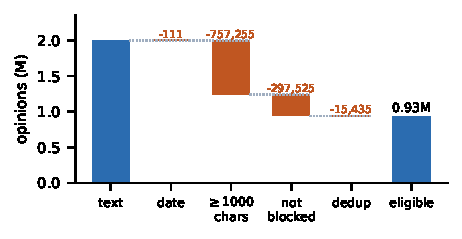
\includegraphics[width=0.88\columnwidth]{generated/fig_funnel.pdf}
\caption{Eligibility funnel. Each bar is the count surviving one criterion, applied in the order shown; the thousand-character minimum is the largest single reduction.}
\label{fig:funnel}
\end{figure}

\subsection{Text} Opinions are stored in several markup flavours. We take the
first non-empty field in a fixed precedence order and strip markup, recording
which field supplied the text so that source composition can be reported by
period. Appendix \ref{app:text} gives the precedence and the composition.

\section{Measuring Non-Resolution at Population Scale}
\label{sec:prev}

\subsection{The frozen dictionary} Candidate generation uses thirteen
expressions, fixed before annotation and unchanged afterwards, listed in Table
\ref{fig:trigger}. Its SHA-1 is \texttt{\DictSHA}. Patterns tolerate a few
intervening words, so ``need not now decide'' is captured alongside the bare
form. One expression is operationalized rather than matched literally. The design
names the stem \emph{reserve}, which in appellate prose is dominated by senses
unrelated to non-resolution, so the pattern requires it to govern a word denoting
a legal question or a deferral.

\subsection{Lexical prevalence is candidate generation, not the measurement} A
count of opinions containing these expressions is not an estimate of judicial
avoidance. It is an upper bound on one observable form of it, inflated by
passages describing other courts and deflated by courts that leave issues open in
ordinary prose. We report it because it fixes the sampling frame and because it
is a population census rather than a sample. For a stratum of $N$ eligible
opinions of which $k$ contain at least one expression we report
\begin{equation}
\hat{\pi}=k/N \quad\text{with}\quad
\hat{\pi}^{\,w}=\frac{k+z^{2}/2}{N+z^{2}},
\end{equation}
the Wilson centre \citep{wilson1927probable}, giving an interval even though the
population is enumerated, because the expression is a noisy proxy for the
practice rather than a sample from it. \S\ref{sec:models} and Appendix
\ref{app:recall} quantify both errors.

\subsection{Analysis hierarchy, fixed in advance} A corpus this size supports a
great many regressions, so the order of questions was fixed before the benchmark
was drawn. Three primary results: whether models separate \textsc{decided} from
\textsc{unresolved}, whether wider context helps, and what fraction of
unresolved issues are later ascribed greater decisional force. Five secondary
questions were pre-specified, covering court level, era, opinion type,
precedential status, and citation volume. Everything else is exploratory and
labelled as such.

\IfFileExists{generated/tab_prev_court_full.tex}{\input{generated/tab_prev_court_full}}{}


\subsection{What the population looks like} Figure \ref{fig:funnel} gives the eligibility funnel. Of \NScanned{} opinion records in the bulk table,
\NFedApp{} belong to the fourteen courts and carry extractable text, and
\NEligible{} survive the eligibility criteria. The largest single reduction is
the thousand-character minimum, which removes short orders and judgment entries;
Supreme Court records account for a disproportionate share of these, because
orders-list entries are stored as opinions. Deduplication removes a further
tranche of records that are the same opinion ingested from more than one source.

\subsection{How often courts say they are not deciding} \NWithTrigger{} eligible
opinions, or \Prevalence{}, contain at least one of the thirteen expressions,
with \NOccurrences{} occurrences in total across \NWordsBn{} billion words.
Figure \ref{fig:trigger} breaks this down by expression and Table
\ref{tab:prevcourt} by court. The rate is not uniform, running from
\CourtLoRate{} in the \CourtLo{} to \CourtHiRate{} in the \CourtHi{}.


\begin{figure}[t]
\centering
\IfFileExists{generated/fig_time.pdf}{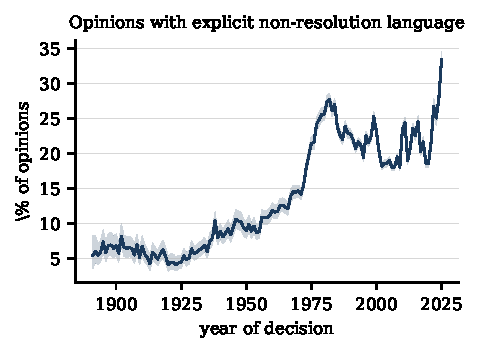
\includegraphics[width=0.88\columnwidth]{generated/fig_time.pdf}}{\fbox{\parbox{0.9\columnwidth}{\centering\vspace{2em}[figure pending]\vspace{2em}}}}
\caption{Share of eligible federal appellate opinions containing at least one
frozen dictionary expression, by year of decision, with Wilson intervals. Years
with fewer than 150 eligible opinions are omitted.}
\label{fig:time}
\end{figure}

 Figure \ref{fig:time} and Table \ref{tab:prevperiod} give
the temporal picture. Both the opinion-level rate and the rate per hundred
thousand words are reported, because opinion length is not constant across eras
and an opinion-level rate alone confounds the two. The corpus itself changes over
this span, in coverage, in digitization source, and in the share of unpublished
dispositions, so the series should be read as a property of the available record
rather than as a clean measurement of judicial behaviour over two centuries.

Opinion type and precedential status were named as secondary analyses before the corpus was built; Appendix \ref{app:prev} reports both.


\begin{figure}[t]
\centering
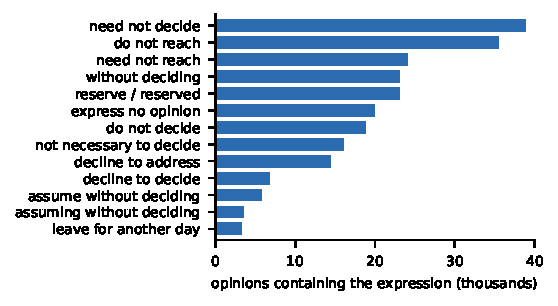
\includegraphics[width=\columnwidth]{generated/fig_trigger.pdf}
\caption{Opinions containing each of the thirteen frozen expressions. T08 and T09 are subsets of T07 by construction.}
\label{fig:trigger}
\end{figure}

\section{Building the Benchmark}
\label{sec:bench}

If the negative class is
passages without a trigger, the task reduces to phrase recognition and
any result is about the dictionary rather than about disposition. Three moves
address this.

\subsection{Matched controls}
For each trigger-bearing opinion we draw a control opinion containing no
dictionary expression anywhere, matched on court, period, opinion type, and
length decile, and locate an issue inside it. Two locators are used: a holding
cue (\textsc{ctrl\_hold}) and a neutral marker naming an issue without
indicating how it came out (\textsc{ctrl\_rand}), so the benchmark stands
independent of the assumption that decided issues are the ones near ``we
hold.''

\subsection{Adversarial strata}
Two structural flags identify passages where the dictionary is likely to
mislead. H1 marks a trigger whose subject is plausibly another institution or
that sits inside a quotation. H2 marks a trigger followed later in the same
opinion by a holding sentence about the same proposition, the shape of a court
that says it need not decide and then decides. Neither flag assigns a label;
both are sampling strata, and annotation settles what the passage does.

\subsection{Neutral issue statements}
Each item carries a statement of the proposition at stake, constructed so it
cannot leak the answer: any dictionary expression or holding cue is cut before
the statement is kept. Appendix \ref{app:issue} gives the procedure and the
\ExtractYield{} yield.

\IfFileExists{generated/tab_stratum_full.tex}{\begin{table}[t]
\centering\small
\begin{tabular}{lrrrr}
\toprule
stratum & dec. & unres. & unclear & \% unres. \\
\midrule
CTRL\_HOLD & 72 & 0 & 1 & 0.0 \\
CTRL\_RAND & 14 & 0 & 16 & 0.0 \\
H1 & 10 & 57 & 31 & 85.1 \\
H2 & 6 & 59 & 0 & 90.8 \\
PLAIN & 5 & 83 & 10 & 94.3 \\
\bottomrule
\end{tabular}
\caption{Annotated labels by sampling stratum. The last column excludes \textsc{unclear}.}
\label{tab:stratum}
\end{table}
}{}


\subsection{Sampling and splits} \NDrawn{} items were drawn with at most one per
opinion, so context windows never overlap and splits are disjoint at the opinion
level. Allocation across strata follows the pilot (Appendix \ref{app:pilot}).
Splits are nested and fixed in order: every item from \HeldOutCourts{} forms the
court-held-out condition, then every remaining item filed in \TemporalCut{} or
later forms the temporal condition, and what is left is split at random into test
and development. Only the development portion was used to fit anything.

\subsection{Annotation} \NAnnotated{} items were annotated under the frozen
guideline, \NUnclear{} of them \textsc{unclear}, leaving \NBench{} with a
usable binary label. Items were presented in a fixed random order ignoring
stratum, split, court, and period, so the annotated set is a random subsample of
what was drawn. Table \ref{tab:stratum} gives labels by stratum.


\section{Can Models Tell?}
\label{sec:models}

\IfFileExists{generated/tab_models_full.tex}{\input{generated/tab_models_full}}{}


\subsection{Systems} Five are compared at four context widths: the frozen
dictionary as a floor; TF-IDF with logistic regression and two fine-tuned
encoders, supervised on the \NDev{}-item development split; a zero-shot open
model, \LLMName{}, scored by the likelihood of the two label continuations so it
never generates; and a classifier seeing only the issue statement, as a leakage
control. One system is deliberately absent: a frontier model would be the natural
comparison, but the only one available here also produced the labels, and a
system evaluated against its own annotations measures nothing.

\subsection{The pooled lexical score is an artefact of our sampling} The frozen
dictionary reaches macro-$F_1$ of \LexF{} on the random test set, which is not a
difficulty measure. Every window is centred on the anchor, so a trigger-bearing
item contains its trigger in every window and a control item contains none. The
rule reduces to ``is this item from the trigger family'': its score is fixed by
the stratum quotas and cannot vary with context width.

\subsection{Supervised systems beat the dictionary where it was built to fail}
On H1, built so the expression is present but is not this court announcing its
own non-resolution, the rule reaches \LexHOne{} while the sparse model reaches
0.947; it also edges the rule on \textsc{plain} (0.962 against 0.942). The
dictionary's pooled advantage comes entirely from the control strata, where it is
correct by construction. The encoders show the pattern more strongly: the best
reaches \BestF{} on the random test set, and on the court-held-out condition
legal-bert reaches 0.975 against the rule's 0.917.

It appeared as the development split
grew, so we measured it directly. Figure \ref{fig:lc} resamples training subsets
of increasing size and evaluates each on the held-out H1 items. Accuracy rises
monotonically, the spread across resamples narrows to nothing, and the share of
subsets beating the dictionary goes from none at 45 items to all of them at
\NDev{}, crossing over near \LCCross{}. That is the shape of a learning curve
rather than of noise, and it says the benchmark is nowhere near saturated.

\begin{figure}[t]
\centering
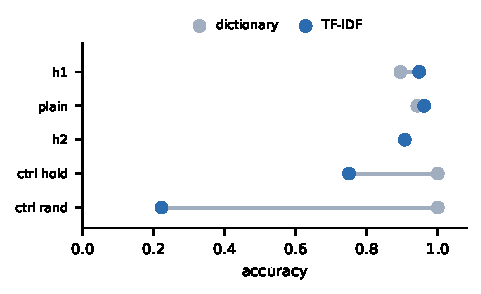
\includegraphics[width=0.88\columnwidth]{generated/fig_strata.pdf}
\caption{Accuracy by sampling stratum at the anchor sentence. The dictionary is at ceiling on the controls by construction; the informative comparison is H1.}
\label{fig:strata}
\end{figure}

\subsection{Context helps up to a point and then hurts} For a window $w$ we
estimate, against the anchor sentence $w_0$,
\begin{equation}
\Delta(w)=F_1\!\left(y,\hat{y}_w\right)-F_1\!\left(y,\hat{y}_{w_0}\right),
\end{equation}
resampling the same items for both conditions, so the comparison is paired and
isolates the window. Table \ref{tab:context} reports it. Widening to $\pm256$
characters costs nothing measurable on the random test set ($-0.014$, 95\% CI
$[-0.110, 0.076]$). Widening further is costly and the effect is clear:
$\pm1024$ costs $-0.245$ and $\pm4096$ costs \CtxWorstDelta{} (95\% CI
$[-0.421, -0.167]$). The zero-shot model traces the same curve, from
\LLMSentF{} at the sentence to \LLMWideF{} at its widest window.

The reading we prefer is that the disposition of one proposition is marked
locally, and that a window wide enough to hold a second issue introduces its
disposition as noise. That is a statement about fixed-window models rather than
about context in principle. A system that locates the later holding sentence rule
L1-3 turns on, rather than consuming everything around it, is left to future
work.


\begin{figure}[t]
\centering
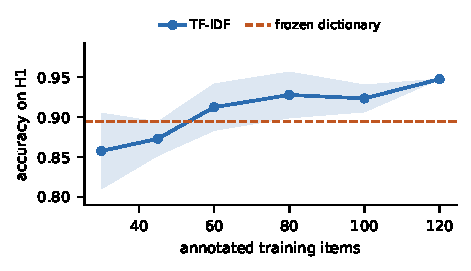
\includegraphics[width=0.82\columnwidth]{generated/fig_lc.pdf}
\caption{Learning curve on the adversarial stratum. Each point resamples twelve training subsets; bars are one standard deviation.}
\label{fig:lc}
\end{figure}

\subsection{Three checks} The issue-only classifier reaches \IssueOnlyF{}
macro-$F_1$ against a majority baseline of 0.392, intervals barely overlapping.
Every dictionary expression and holding cue is stripped from a statement before
it is kept, so this is not lexical leakage but subject matter: which questions
courts decline to reach correlates with what they are about. Part of what looks
like reasoning is available from the topic alone.

Re-annotating \NHumanAbl{} items with only the anchor sentence, the label matches
the full-context label \HumanAgree{} of the time, and every flip falls in H1 and
\textsc{ctrl\_hold}. What changes most is the willingness to answer, abstention
rising from \HumanUnclearFull{} to \HumanUnclearSent{}. For a person as for a
model, context buys confidence more than accuracy.

Courts also label each other. A parenthetical reading ``(declining to decide
whether $X$)'' asserts that the cited case did not resolve $X$, and we harvest
\NCharTight{} such characterizations. They serve as a resource rather than as
validation, since if a later court says \emph{Smith} held $X$ and we say
\emph{Smith} left $X$ open, either our label is wrong or the later court has
overstated \emph{Smith}, and the disagreement is consistent with both. Appendix \ref{app:errors} works through
the cases that separate the systems, selected by a fixed rule rather than by
hand.

\section{What Happens Next to an Unresolved Issue}
\label{sec:long}

Annotating citation chains one at a time does not scale. Of citing passages that
survive a content-word filter, \OffIssueRate{} are still about something other
than the issue, so a usable observation costs roughly ten annotations. Instead we
measure the phenomenon the way \S\ref{sec:prev} measures prevalence, with frozen
dictionaries applied to the whole corpus.

\subsection{Matching propositions, not positions} Asking whether a
non-resolution expression sits near the characterized passage is cheap but wrong:
of \NProxyCheck{} flagged cases only \NProxyGood{} were genuine, the expression
usually governing a neighbouring question (Appendix \ref{app:layer2}). Comparing propositions works. Writing
$C(x)$ for the content words of a text, we match the origin's issue statement $q$
against the later court's characterization $c$ when
\begin{equation}
J(q,c)=\frac{|C(q)\cap C(c)|}{|C(q)\cup C(c)|}\;\geq\;\tau,
\qquad \tau=0.34,
\end{equation}
so both sides of the comparison are propositions rather than positions in a
document. Of \NCharTight{} characterizations only
\NIMMatched{} clear the threshold, few enough to hand-verify each:
\NIMGenuine{} are genuine, \NIMPrec{} precision against \ProxyPrec{}, over
\NIMDistinct{} propositions.

\begin{figure}[t]
\centering
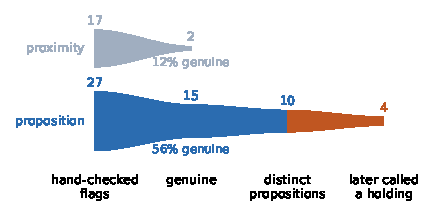
\includegraphics[width=0.74\columnwidth]{generated/fig_escal.pdf}
\caption{Attrition under the two matching strategies. Ribbon thickness is the
count at each stage, so the first taper is the verified precision. The orange
tail is the case series.}
\label{fig:escal}
\end{figure}

\subsection{What the verified cases show} Among those \NIMDistinct{}
propositions, each one a question the originating court demonstrably declined to
decide, \NIMEsc{} are described by a later court as something that court held.
The majority are reported accurately, with the later court repeating the
reservation, as when one opinion notes that \emph{Davis} reserved the question
whether a request for counsel can be rendered ambiguous by preceding events.

Writing $S(o_1,q)\in\{L_0,\dots,L_3\}$ for the status a later opinion $o_1$
ascribes to proposition $q$ and $S_0(q)$ for what the origin did, the quantity of
interest is
\begin{equation}
\Pr\!\left[S(o_1,q)=L_3 \mid S_0(q)=\textsc{unresolved}\right],
\end{equation}
the chance that a question a court declined to decide is later called its
holding. This is a case series and not a rate. Ten propositions cannot support an
interval, and the threshold selects for verbatim quotation and so for the cases
most likely to be characterized accurately, a bias against the phenomenon. It
establishes that escalation occurs and that issue matching, not data, is the
constraint. Appendix \ref{app:layer2} elaborates.



\section{Conclusion}
\label{sec:conclusion}
Across \NEligible{} eligible federal appellate opinions, \Prevalence{} contain
at least one of thirteen frozen expressions of non-resolution. Declining to
decide is not marginal. It is routine, announced in a vocabulary that has held
its shape for a century, and rising in every era we can measure.

Pooled, the dictionary looks unbeatable, but that is fixed by the sampling. Per
stratum the systems separate: on H1 the sparse model reaches 0.947 against
\LexHOne{}, and on the court-held-out condition an encoder beats it outright.
Context helps to \(\pm256\) characters and then degrades. The task is therefore
not phrase recognition, and more text without a way to know what to look for in
it makes systems worse.

For the empirical study of courts, the consequence is that a citation is a
coarser instrument than it is usually taken to be. Network accounts of precedent
read an edge as evidence of the cited opinion's authority
\citep{fowler2007network, black2013citation}, but an edge ascribing a holding to
an opinion that expressly declined to reach the question means something
different from one that follows a real holding, and the edge does not distinguish
them. In \NIMEsc{} of \NIMDistinct{} hand-verified propositions a later court
described as settled what the originating court had reserved. Ten cases are a
case series and not a rate, but they show the failure is real, and an instrument
of this kind is what makes it countable at all.

The same gap runs downstream, since retrieval and summarization over case law
inherit the assumption that a proposition attached to a citation was decided
where it was cited. Separating disposition from discussion is a prerequisite for
legal information systems, not an application of them.


% Content ends here. Everything below begins on the next page, so the
% eight-page content limit is enforced by the document rather than by eye.
\clearpage

\section*{Limitations}

\subsection*{Who produced the labels} A single annotator applied the frozen
guideline, so the labels carry no inter-annotator agreement statistic. A blind
second pass over already-labelled items, shown in a different order with the
first-pass labels withheld, reproduced them exactly (27 of 27, $\kappa=1.00$). We
report the figure and rest little on it, since perfect self-agreement is as
consistent with an annotator recognising passages seen earlier as with a
guideline that admits one reading. The quantity we do rest on is the
within-annotator context ablation (\S\ref{sec:models}), which measures how far
the same annotator's decisions depend on material outside the anchor sentence.
Whether two trained lawyers would agree on these labels is a question for a
follow-up study with a practitioner panel.

The annotator is a language model, which places it in the same family as some of
the systems under evaluation. Two design choices contain the circularity. The
supervised baselines are trained from the labels but are architecturally
independent of the label source, and they carry the context-scaling result. The
zero-shot baseline is a small open model that had no part in producing the
labels, saw no guideline, and was scored by label-token likelihood, so it is
independent of them. A frontier model evaluated against its own annotations would
report agreement with itself, so we omit that comparison. The escalation results
in \S\ref{sec:long} rest on the same labels.

\subsection*{Benchmark and split sizes} Annotation produced \NBench{} usable
labels, \NDev{} for development and 104, 36, and 46 for the three held-out
conditions. At that size, differences of a few macro-$F_1$ points sit inside the
noise, and the temporal condition carries wide intervals. The two comparisons we
rest on are the per-stratum contrast, where the gap between the sparse model and
the dictionary on H1 is large, and the paired context comparison, which is
within-item and therefore better powered than the split sizes suggest. One fact a
reader should weigh is that the separation between supervised systems and the
dictionary emerged as the development split grew, having been absent at half this
annotation scale. That is the signature of an effect that needed data to surface,
and it is also a reason to rerun the benchmark at several thousand items.

The leakage control reaches \IssueOnlyF{} macro-$F_1$ against a majority baseline
of 0.392, with intervals that barely overlap. Every dictionary expression and
holding cue is stripped from a statement before it is kept, so the signal here is
subject matter rather than lexical leakage of the label. Which questions courts
decline to reach is correlated with what the questions are about, so part of what
a system appears to infer from the passage is available from the topic alone.
Future versions of this benchmark should either match strata on subject matter or
report the issue-only control alongside every headline number, as we do here.

\subsection*{What the dictionary measures} A court can leave an issue open in
ordinary prose. Freezing the thirteen expressions before annotation protects
against tuning them to a result, and the recall audit in Appendix
\ref{app:recall} bounds what they miss by reading a random sample of opinions
containing none of them. Prevalence figures should be read as the rate of
explicitly marked non-resolution. The item frame is scoped the same way. It
admits anchors with a recoverable issue statement, and yield varies across
expressions and, less strongly, across courts, so the benchmark samples anchors
with a recoverable proposition. Appendix \ref{app:issue} reports yield by
stratum so the direction of the loss is visible.

\subsection*{Corpus coverage} CourtListener is broad but uneven. Coverage,
metadata completeness, and text quality vary by court and era, and the same
opinion is sometimes stored more than once from different upstream sources. We
deduplicate and report the eligibility funnel, and a change in measured
prevalence across periods remains partly a change in what was digitized and how.
This is why period-stratified rates appear throughout rather than a single time
series presented as a trend in judicial behaviour.

A citing passage is treated as being about the origin's issue when its content
words overlap the issue statement. That admits false positives, where a later
opinion cites the origin for a neighbouring point sharing vocabulary, and false
negatives, where a later court restates the issue in different words. Annotation
removes the false positives, since off-issue passages are labelled and dropped,
and the false-negative rate is unmeasured.

\subsection*{Scope of the comparison} The comparison between unresolved and
decided issues matches on court, period, opinion length, and citation volume, and
is descriptive. Whether an issue was left open is a judicial choice correlated
with unobservables, including how hard and how contested the issue was, and those
plausibly affect how later courts describe it. We report the contrast as an
association.

Chains require the origin to carry a reporter citation locatable in the citing
text, and are restricted to citing opinions inside the population, so district
and state court treatments fall outside the sample and origins in the most recent
years have had little time to accumulate citations. Both restrictions bias the
chain sample toward older, better-reported, more-cited opinions.

The encoder baselines truncate at 512 tokens and the zero-shot model at 1600,
which caps the widest context condition, so the comparison across context widths
is partly a comparison of how much of the window each architecture uses. The
zero-shot model has 3.8B parameters, and its role here is to show that an
independent model responds to the context manipulation in the same direction. The
study covers English-language United States federal appellate opinions, and
extension to state courts, trial courts, agency adjudication, or other legal
systems remains future work.


\section*{Ethics Statement}

The corpus consists of published judicial opinions, which are public records, and
we add no information about any individual beyond what those opinions already
contain. Opinions name parties, including criminal defendants, immigration
petitioners, and civil litigants. We release passage offsets and opinion
identifiers rather than redistributing text, so that removals and corrections
upstream propagate. The task is descriptive. A system that classifies issue
disposition should not be used to characterize a court's work without review, and
the escalation analysis measures how propositions are described in later
opinions, not whether any court erred. We name no judge in any reported result.

\bibliography{refs}
\bibliographystyle{acl_natbib}

\appendix
\section{Excluded Federal Courts}
\label{app:courts}
CourtListener assigns federal jurisdiction codes to many bodies beyond the
fourteen courts in the population. Every excluded court is listed in the released
artefact \texttt{01\_courts.json}. They fall into four groups: the historical
circuit courts that sat before the Judiciary Act of 1891, appearing under roughly
130 identifiers of the form \texttt{circt*}; abolished or specialized Article I
and Article III courts, among them the Court of Customs and Patent Appeals, the
Court of Claims, and the Court of International Trade; the Foreign Intelligence
Surveillance Court and its Court of Review; and administrative review bodies
whose decisions are published alongside judicial opinions, among them the Board
of Immigration Appeals, the Merit Systems Protection Board, and the Patent Trial
and Appeal Board.

Excluding administrative bodies is a substantive choice. Agency adjudicators use
the same vocabulary of non-resolution, but they are not courts of appeals, their
decisions carry different precedential force, and the citation practices layer
two depends on differ. The historical circuit courts are excluded for a different
reason: their reporting is uneven and their text largely OCR-derived, so a rate
computed over them would measure digitization as much as judicial practice.

\section{Text Extraction}
\label{app:text}

CourtListener stores an opinion's text in whichever markup flavours its upstream
sources supplied. We take the first field with usable content in the order
\texttt{html\_columbia}, \texttt{html\_lawbox}, \texttt{xml\_harvard},
\texttt{html\_anon\_2020}, \texttt{html}, \texttt{plain\_text},
\texttt{html\_with\_citations}. The citation-annotated variant is last because it
injects anchor text into the body. Markup is removed by closing block-level tags
into newlines, deleting remaining tags, unescaping entities, and normalizing
whitespace; character offsets in the released benchmark refer to this normalized
text. Table \ref{tab:textsrc} reports which field supplied the text, by period.
Source composition shifts with period because different digitization projects
covered different eras, which is one reason we report period-stratified rates
rather than a single pooled trend.

\IfFileExists{generated/tab_textsrc_full.tex}{\begin{table*}[t]
\centering\small
\begin{tabular}{lrrrr}
\toprule
field & pre-1990 & 1990-2004 & 2005-2014 & 2015-2026  \\
\midrule
\texttt{html} & 17.2 & 30.1 & 2.3 & 0.0 \\
\texttt{html\_lawbox} & 10.5 & 0.6 & 12.9 & 0.0 \\
\texttt{plain\_text} & 0.0 & 13.3 & 16.8 & 67.7 \\
\texttt{xml\_harvard} & 72.3 & 56.0 & 68.0 & 32.3 \\
\bottomrule
\end{tabular}
\caption{Text source field by period, as a percentage of eligible opinions in that period.}
\label{tab:textsrc}
\end{table*}
}{}


\section{The Frozen Trigger Dictionary}
\label{app:dict}

Figure \ref{fig:trigger} lists the thirteen expressions with
their corpus frequencies. The regular expressions themselves are reproduced
below; they were fixed before annotation and their SHA-1 is \texttt{\DictSHA}.

\IfFileExists{generated/tab_regex_full.tex}{\begin{figure*}[t]
\centering\scriptsize
\begin{verbatim}
T01  need(?:s|ed)?\s+not\s+(?:\w+\s+){0,2}?decide\b
T02  need(?:s|ed)?\s+not\s+(?:\w+\s+){0,2}?reach\b
T03  \bdo(?:es)?\s+not\s+(?:\w+\s+){0,2}?decide\b
T04  \bdo(?:es)?\s+not\s+(?:\w+\s+){0,2}?reach\b
T05  declin(?:e|es|ed|ing)\s+to\s+(?:\w+\s+){0,2}?decide\b
T06  declin(?:e|es|ed|ing)\s+to\s+(?:\w+\s+){0,2}?address\b
T07  \bwithout\s+deciding\b
T08  \bassuming\s+(?:\w+\s+){0,4}?without\s+deciding\b
T09  assum(?:e|es|ed)\s+(?:\w+\s+){0,4}?without\s+deciding\b
T10  express(?:es|ed|ing)?\s+no\s+(?:\w+\s+){0,2}?opinion\b
T11  reserv(?:e|es|ed|ing)\s+(?:\w+\s+){0,3}?(?:question|questions|issue|issues|matter|judgme
    nt|decision)\b|reserv(?:e|es|ed|ing)\s+(?:\w+\s+){0,3}?for\s+another\s+(?:day|case)\b
T12  leav(?:e|es|ing)\s+(?:\w+\s+){0,4}?(?:for|to|until)\s+another\s+(?:day|case|occasion)\b
T13  \b(?:not|un)\s*necessary\s+to\s+(?:decide|reach|resolve|address)\b
\end{verbatim}
\caption{The thirteen frozen expressions as regular expressions, matched case-insensitively over whitespace-normalized text.}
\label{tab:regex}
\end{figure*}
}{}


T08 and T09 are proper subsets of T07 by construction. They are retained because
the design names them separately, and a passage matching several expressions is
counted once in opinion-level rates while keeping every identifier. T11 is the
only expression not matched as written, for the reason given in
\S\ref{sec:prev}.

\section{Issue Statement Extraction}
\label{app:issue}

An item needs a statement of the proposition at stake that does not reveal the
answer. We derive it from the sentence containing the anchor rather than from a
fixed character budget, which stops the clause running into whatever the court
said next.

The procedure takes the material following the anchor within the anchor's
sentence, deletes reporter citations and signals, and looks for a
\emph{whether}-complement within the first sixty characters. If none is present
but the clause opens with a complementizer or a preposition taking a
propositional object, it is rewritten as a \emph{whether}-clause. If it opens
with neither, it is kept as a noun phrase, but only when its first token is not a
verb, negation, conjunction, or pronoun, since those signal a fragment rather
than a statement of an issue. Where the trigger closes its own sentence, the
material before the anchor is used instead, and only when that material itself
names the issue with \emph{whether}, \emph{the question of}, or \emph{the issue
of}. Two filters run last. Any dictionary expression or holding cue in the
candidate statement is cut, which is what allows the claim that no issue
statement contains one, and statements with fewer than three content words, or
more than forty percent non-alphabetic, are rejected as extraction debris.

Rejection is not random. An anchor with no extractable issue statement does not
enter the frame, so the benchmark is a sample of anchors with a recoverable
proposition rather than of all anchors. Table \ref{tab:extract} reports the yield
by expression and by court so that the direction of any bias is visible.

\IfFileExists{generated/tab_extract_full.tex}{\begin{table}[t]
\centering\small
\begin{tabular}{lrrr}
\toprule
id & anchors & with issue & yield (\%) \\
\midrule
T01 & 49,640 & 34,951 & 70.4 \\
T02 & 30,909 & 16,737 & 54.1 \\
T03 & 22,309 & 15,820 & 70.9 \\
T04 & 45,401 & 25,678 & 56.6 \\
T05 & 8,144 & 5,871 & 72.1 \\
T06 & 21,004 & 10,165 & 48.4 \\
T07 & 30,894 & 23,189 & 75.1 \\
T08 & 4,718 & 3,420 & 72.5 \\
T09 & 7,779 & 5,663 & 72.8 \\
T10 & 24,641 & 17,710 & 71.9 \\
T11 & 34,080 & 15,684 & 46.0 \\
T12 & 3,508 & 1,826 & 52.1 \\
T13 & 18,876 & 11,670 & 61.8 \\
\bottomrule
\end{tabular}
\caption{Issue-statement extraction yield by expression.}
\label{tab:extract}
\end{table}
}{}


\section{Annotation Guidelines}
\label{app:guide}

The guidelines below are reproduced verbatim from the frozen protocol. Version
1.0 was drafted before the pilot; version 1.1 incorporates the single revision
the design permits, made once after the pilot and before any main-sample
annotation.

\begin{quote}\scriptsize\begin{verbatim}
TASK. You are given a legal issue and a passage from
  a United States federal
appellate opinion. Decide whether the opinion
  resolved that issue.

LABELS.
  DECIDED     The authoring court resolved the
    issue. It stated a holding, a
              conclusion, or a
                determination on the
                issue, whether or not
                that
              resolution was necessary
                to the judgment, and
                whether or not it
              was later characterized
                as dictum.
  UNRESOLVED  The authoring court did not resolve
    the issue for itself.

If and only if the label is UNRESOLVED, assign one
  sublabel.
  AVOIDED     The court declined to reach the
    issue because some other ground
              disposed of the case or
                the claim. Typical
                form: "because we
              affirm on qualified
                immunity grounds, we
                need not decide
                whether
              the search was lawful."
  ASSUMED     The court proceeded on a stated
    assumption about the issue and
              resolved the case on
                other grounds, so that
                the assumption did
              no independent work.
                Typical form:
                "assuming without
                deciding
              that the statute reaches
                this conduct, the
                evidence is
              insufficient."
  RESERVED    The court expressly held the issue
    open for future resolution,
              signalling that it
                remains available.
                Typical form: "we
                leave for
              another day whether
                Chevron survives in
                this context."

DECISION RULES.
  L1-1  ATTRIBUTION. The label describes what THIS
    opinion did. Language about
        what a different court did, whether
          a lower court, a sister circuit,
          or
        the Supreme Court, does not by
          itself make this opinion's
          disposition
        UNRESOLVED. "The district court
          concluded it need not decide X"
          tells
        you about the district court. Read
          on to see what this court did.
  L1-2  UNIT. In a cluster containing a majority
    opinion and separate opinions,
        each opinion is its own unit. A
          dissent that would decide an issue
          the
        majority avoided is DECIDED for the
          dissent and UNRESOLVED for the
        majority.
  L1-3  LATER RESOLUTION CONTROLS. A court may
    write "we need not decide X" and
        then decide X anyway, in the same
          opinion, in an alternative
          holding, in
        a footnote, or in a later section.
          Where the opinion does resolve the
        issue somewhere, the label is
          DECIDED. A court's
          characterization of
        what it need not do controls only
          where no independent resolution
        follows.
  L1-4  ASSUMPTION THAT DOES WORK. If the court
    assumes a proposition and the
        assumption is then treated as
          settled for the remainder of the
          analysis
        in a way that determines the
          outcome, the label remains
          UNRESOLVED and
        the sublabel is ASSUMED. Assuming a
          proposition is not deciding it,
          even
        when the assumption drives the
          result.
  L1-5  NO TRIGGER REQUIRED. UNRESOLVED does not
    require any particular phrase.
        A court can leave an issue open in
          ordinary prose.
  L1-6  PARTIAL RESOLUTION. The unit is the
    proposition named in the issue
        statement, not the broader legal
          question it belongs to. If the
          court
        resolves the anchored proposition
          but leaves a neighbouring one
          open,
        the label is DECIDED. If the court
          resolves a neighbouring
          proposition
        but leaves the anchored one open,
          the label is UNRESOLVED.
  L1-7  REMANDS. An issue remanded for the
    district court to address in the
        first instance is UNRESOLVED,
          sublabel AVOIDED, unless the
          appellate
        court also states the governing rule
          and applies it.
  L1-8  ABSTAIN. If the passage is too corrupt,
    too truncated, or too ambiguous
        to support either label, output
          UNCLEAR rather than guessing.
  L1-9  ISSUES THIS OPINION NEVER TAKES UP.
    Sometimes the only reason an issue
        is in front of you is that the
          opinion mentioned, in a
          parenthetical or
        in a description of some other
          court's work, that a different
          court did
        not decide it, and this opinion
          never reaches the issue in its own
        right. That is neither DECIDED nor
          UNRESOLVED for this opinion.
          Output
        UNCLEAR. This rule does not apply
          where the opinion goes on to
          engage
        with the issue itself: there, L1-1
          and L1-3 govern.
\end{verbatim}\end{quote}

\noindent Version 1.1. The single permitted revision after the pilot, and the layer-two and issue-statement guidelines, are in the released package.


\section{Pilot Study and Protocol Revision}
\label{app:pilot}

The pilot ran on a preliminary frame built from a leading portion of the bulk
opinion table, before the full pass was committed to. Its purpose was to find
out whether the guideline could be applied at all, whether the controls behaved,
and which strata were worth sampling heavily. Sixty items were annotated. Pilot
items are not part of the benchmark and no pilot label appears in any result.

\subsection{What the pilot showed} Labels fell out by stratum as follows:
\textsc{ctrl\_hold} 12 \textsc{decided} and 0 \textsc{unresolved};
\textsc{plain} 19 \textsc{unresolved} and 1 \textsc{decided};
H2 8 \textsc{unresolved} and 2 \textsc{decided};
H1 5 \textsc{unresolved}, 5 \textsc{decided}, and 5 \textsc{unclear}.

Three things follow. The holding-cue control behaves as intended and is not
contaminated. The \textsc{plain} stratum is nearly degenerate: a trigger with no
structural complication almost always does mean the court left the issue open,
which is why a keyword rule scores as well as it does and why that score means
little. The H1 stratum is close to an even split, so it is where the task
actually lives, and the sample was reallocated toward it. This reallocation
changes only how many items are drawn per stratum. Label definitions and stratum
definitions were fixed before the pilot and held throughout.

\subsection{The one protocol revision} Version 1.0 of the guideline had no rule
for a passage whose only trigger sits inside a parenthetical or a description of
another court's work, on a question the present opinion never reaches in its own
right. A citation noting that the Supreme Court declined to decide whether an
airport user fee was excessive tells you nothing about the disposition of the
Federal Circuit opinion that cites it, and forcing a choice between
\textsc{decided} and \textsc{unresolved} would have manufactured a label. Rule
L1-9 routes these to \textsc{unclear}. It uses an existing label; it adds none.
This is the single revision the design permits, it was made once, before any
main-sample annotation, and the changelog is reproduced in
Appendix~\ref{app:guide}.

\subsection{Three pipeline defects the pilot exposed} These concern candidate
construction, not the guideline. The pattern flagging a trigger as plausibly
describing another institution was case-sensitive, matching ``the district
court'' but missing ``the District Court,'' which appellate opinions write about
as often; it now also recognizes ``the court held'' and its near neighbours. The
annotator was shown a later holding sentence only for items already flagged H2,
though Rule L1-3 turns on precisely that passage, so an H1 item whose opinion
later resolved the issue was unanswerable rather than hard; the sentence is now
shown whenever one exists outside the displayed window. And ``our holding'' was
a control locator, but in the pilot it pointed at a named prior case rather than
the present disposition every time it fired, so it was dropped.

\subsection{What the pilot did not do} It was not used to adjust any label
boundary. The trigger dictionary was frozen before the pilot and is unchanged;
in particular, the pilot surfaced two recurring dictionary false positives, and
neither was patched. One is the statutory-scope reading of \emph{reach}, as in
``the shipment clause does not reach shipments between the continental States,''
which is a holding about a statute rather than a non-resolution. The other is a
line-break artefact in the source text that splits \emph{preserving} into
\texttt{P} and \texttt{reserving}, which then matches T11. Both stay in, are
labelled \textsc{decided} by the guideline, and are counted against the
dictionary in \S\ref{sec:models}.


\section{Dictionary Recall Audit}
\label{app:recall}

The frozen dictionary bounds what candidate generation can find. It says nothing
about non-resolution expressed in language outside it. To bound that, we drew a
random sample of eligible opinions containing no dictionary expression and read
them for issues the court discussed and left unresolved.

Reading whole opinions at random is a weak audit. A non-resolution can sit
anywhere in forty pages, most opinions contain none, and an annotator who has
internalized the dictionary is primed to see the vocabulary it already
covers.

We use a second, deliberately wider probe list instead. Fifteen expressions
outside the frozen dictionary were written after the fact and run over a random
sample of \RecallSampled{} opinions the dictionary called clean. The probe is
confined to this audit and enters neither candidate generation, the benchmark,
nor any prevalence figure.

\RecallHit{} of clean opinions contain at least one probe expression. Table
\ref{tab:recall} gives the breakdown. What that figure bounds needs stating
carefully. It is a measure of \emph{lexical} coverage, not of missed
non-resolution. Some probe hits are genuine, as in a Seventh Circuit opinion
that writes ``Volkswagen does not raise this argument and we do not resolve
it,'' and then says the question ``remains unsettled.'' Others are the same
statutory-scope reading of \emph{reach} and \emph{address} that already
contaminates the frozen dictionary, where the court is saying what a statute
covers rather than what it declined to decide. Annotating a sample of probe hits would be needed to convert the probe rate
into an estimate of missed non-resolution, so we report it as a coverage
figure.

The largest omission is the \emph{address}, \emph{consider}, \emph{resolve}
family. The frozen dictionary contains \emph{need not decide} and \emph{need not
reach} but not \emph{need not address}, and \emph{decline to address} but not
\emph{decline to consider}. The design named thirteen expressions and they were
frozen before annotation, so the gap stands rather than being patched. The pilot
had already flagged one instance, in a control opinion reading ``we need not
address the government's contention'' that was nonetheless admitted to the
zero-trigger pool.

Two consequences follow for how the paper's numbers should be read. Population
prevalence in \S\ref{sec:prev} measures explicitly marked non-resolution using
one fixed vocabulary, and a wider vocabulary would find more, so it is a floor
rather than an estimate of the phenomenon. And the control pool is contaminated
in a known direction, since some opinions admitted as trigger-free do contain
unresolved issues expressed in language outside the dictionary. That
contamination makes the controls harder rather than easier, so it works against
every reported separation rather than for it.

\IfFileExists{generated/tab_recall_full.tex}{\input{generated/tab_recall_full}}{}




\section{Full Prevalence Tables}
\label{app:prev}

\begin{table*}[t]\centering\small
\begin{tabular}{lrrrr}
\toprule
court & 1990-2004 & 2005-2014 & 2015-2026 & pre-1990 \\
\midrule
Supreme Court & 28.88 & 30.96 & 34.35 & 14.78 \\
1 Cir. & 28.67 & 31.66 & 39.27 & 19.87 \\
2 Cir. & 25.66 & 19.77 & 28.40 & 15.42 \\
3 Cir. & 34.48 & 21.23 & 25.60 & 20.21 \\
4 Cir. & 12.30 & 11.62 & 11.85 & 13.00 \\
5 Cir. & 22.07 & 20.69 & 20.02 & 15.01 \\
6 Cir. & 14.63 & 24.52 & 26.73 & 10.87 \\
7 Cir. & 19.80 & 16.86 & 18.77 & 17.33 \\
8 Cir. & 17.43 & 19.17 & 18.60 & 12.82 \\
9 Cir. & 20.24 & 17.72 & 21.17 & 18.68 \\
10 Cir. & 21.11 & 27.65 & 32.08 & 12.23 \\
11 Cir. & 28.97 & 19.78 & 23.54 & 24.72 \\
D.C. Cir. & 29.92 & 25.94 & 32.50 & 19.18 \\
Fed. Cir. & 16.59 & 20.22 & 24.93 & 17.89 \\
\bottomrule
\end{tabular}
\caption{Share of opinions containing at least one dictionary expression, by court and period.}\label{tab:cp}
\end{table*}

\begin{table}[t]\centering\small
\begin{tabular}{lrrr}
\toprule
type group & $N$ & $k$ & \% \\
\midrule
majority/lead & 864,804 & 169,373 & 19.59 \\
other & 1,664 & 101 & 6.07 \\
separate & 61,786 & 6,136 & 9.93 \\
\bottomrule
\end{tabular}
\caption{By opinion type.}\label{tab:type_group}
\end{table}

\begin{table}[t]\centering\small
\begin{tabular}{lrrr}
\toprule
precedential status & $N$ & $k$ & \% \\
\midrule
Errata & 104 & 3 & 2.88 \\
Published & 767,586 & 160,008 & 20.85 \\
Relating-to & 552 & 21 & 3.80 \\
Unknown & 3,291 & 1,139 & 34.61 \\
Unpublished & 156,706 & 14,439 & 9.21 \\
\bottomrule
\end{tabular}
\caption{By precedential status.}\label{tab:precedential_status}
\end{table}


\begin{figure}[t]
\centering
\IfFileExists{generated/fig_heat.pdf}{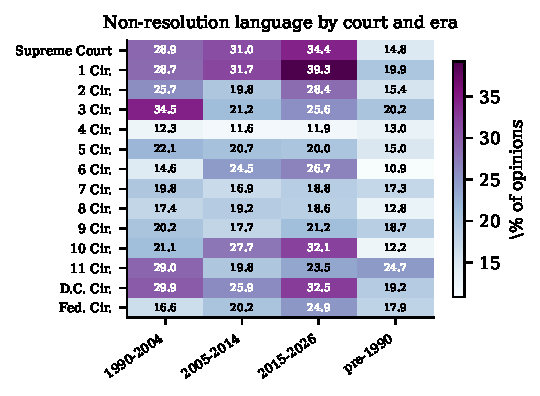
\includegraphics[width=\columnwidth]{generated/fig_heat.pdf}}{}
\caption{Share of eligible opinions containing at least one frozen dictionary
expression, by court and period. Cells with fewer than 150 eligible opinions are
left blank rather than plotted as noise.}
\label{fig:heat}
\end{figure}

\section{Cross-Check Against the Search Index}
\label{app:api}

The bulk release and the public CourtListener search index are built from the
same database but refreshed on different schedules and tokenized differently.
Querying the index for the thirteen literal phrases, restricted to the fourteen
courts, gives an estimate of how many opinions contain each expression that is
independent of our text extraction, markup handling, and field precedence.

Three hundred count queries were issued against the v4 search endpoint: a
denominator for each of the fourteen courts, a denominator for each court and
period, and a count for each of the thirteen literal phrases, both per court and
pooled. No opinion text was retrieved.

Two differences from the bulk pipeline are expected and neither is a defect.
The index counts opinions as the search system stores them, while our
denominator counts opinions surviving the eligibility criteria of
\S\ref{sec:corpus}, which remove short orders and duplicates; the index
denominator is therefore the larger of the two. And the index matches literal
phrases, while the frozen dictionary tolerates a few intervening words and
constrains T11, so the two counts are not measuring the same event. The
comparison is useful precisely because the two disagree in known directions: a
large unexplained gap would indicate that markup handling or field precedence
was losing text, and a close match on the shape of the distribution across
courts and expressions indicates that it is not.

The pooled index count over the thirteen literal phrases restricted to the
fourteen courts is 108{,}669 opinions against a denominator of
\ApiTotal{} indexed opinions, an implied rate of 7.8\%. Ranking the expressions
by frequency, the index and the bulk corpus agree on the ordering of the top
group, with \emph{need not decide} first in both.

\IfFileExists{generated/tab_api_full.tex}{\input{generated/tab_api_full}}{}



\section{Supplementary Tables}
\label{app:supp}
\IfFileExists{generated/tab_context_full.tex}{\input{generated/tab_context_full}}{}

\IfFileExists{generated/tab_prev_period_full.tex}{\input{generated/tab_prev_period_full}}{}

\IfFileExists{generated/tab_paths_full.tex}{\input{generated/tab_paths_full}}{}

\IfFileExists{generated/tab_tailpair_full.tex}{\begin{table*}[t]
\centering
\begin{minipage}[t]{0.46\textwidth}
\centering\small
\begin{tabular}{lrr}
\toprule
split & $n$ & \% unresolved \\
\midrule
COURT & 54 & 57.4 \\
DEV & 143 & 53.8 \\
TEMPORAL & 44 & 54.5 \\
TEST & 123 & 54.5 \\
\bottomrule
\end{tabular}
\captionof{table}{Evaluation splits. They are disjoint at the opinion level and only \textsc{dev} was used for fitting.}
\label{tab:splits}
\end{minipage}\hfill
\begin{minipage}[t]{0.50\textwidth}
\centering\small
\begin{tabular}{lrr}
\toprule
stratum & $n$ & agreement with full context (\%) \\
\midrule
CTRL\_HOLD & 4 & 75.0 \\
H1 & 11 & 81.8 \\
H2 & 7 & 100.0 \\
PLAIN & 9 & 100.0 \\
\bottomrule
\end{tabular}
\captionof{table}{How often the annotator's sentence-only label matches the label the same annotator gave with the full window. A within-annotator context ablation, not an inter-annotator statistic.}
\label{tab:humanabl}
\end{minipage}
\end{table*}
}{\IfFileExists{generated/tab_splits_full.tex}{\begin{table*}[t]
\centering\small
\begin{tabular}{lrr}
\toprule
split & $n$ & \% unresolved \\
\midrule
COURT & 54 & 57.4 \\
DEV & 143 & 53.8 \\
TEMPORAL & 44 & 54.5 \\
TEST & 123 & 54.5 \\
\bottomrule
\end{tabular}
\caption{Evaluation splits. They are disjoint at the opinion level and only \textsc{dev} was used for fitting.}
\label{tab:splits}
\end{table*}
}{}
\IfFileExists{generated/tab_humanabl_full.tex}{\begin{table}[t]
\centering\small
\begin{tabular}{lrr}
\toprule
stratum & $n$ & agreement with full context (\%) \\
\midrule
CTRL\_HOLD & 4 & 75.0 \\
H1 & 11 & 81.8 \\
H2 & 7 & 100.0 \\
PLAIN & 9 & 100.0 \\
\bottomrule
\end{tabular}
\caption{How often the annotator's sentence-only label matches the label the same annotator gave with the full window. A within-annotator context ablation, not an inter-annotator statistic.}
\label{tab:humanabl}
\end{table}
}{}
}

These are collected rather than placed inline because each is a secondary cut on
a quantity already reported.

\section{Model Details}
\label{app:models}

\subsection{Context conditions} Every system is evaluated under four windows
around the anchor: the anchor's sentence (\textsc{sent}), and $\pm256$,
$\pm1024$, and $\pm4096$ characters. Windows are cut from the normalized text and
whitespace-collapsed. The sentence condition isolates local lexical evidence; the
widest condition is the only one that routinely reaches a later holding sentence
in the same opinion, which is what the H2 stratum requires.

\subsection{Lexical rule} The floor. The frozen dictionary is applied to the
context window and the item is predicted \textsc{unresolved} when any expression
matches. This is not a strawman: it is exactly the procedure that generated the
candidates, and it is what a keyword system would do. Because controls are drawn
from opinions containing no dictionary expression anywhere, the rule is close to
perfect on the \textsc{ctrl} strata by construction, and its overall number is
therefore an optimistic reading of what phrase matching achieves. The strata that
matter are H1 and H2, where the rule is wrong whenever the annotation says the
court's actual disposition runs against the phrase.

\subsection{Sparse baseline} TF-IDF over word unigrams and bigrams, minimum
document frequency two, at most 60{,}000 features, sublinear term frequency,
followed by $\ell_2$-regularized logistic regression with $C=4$ and balanced
class weights. Trained on \textsc{dev} only.

\subsection{Encoders} LEGAL-BERT \citep{chalkidis2020legalbert} and
DistilRoBERTa, fine-tuned for five epochs at learning rate $2\times10^{-5}$,
batch size 16, maximum length 512 tokens, with the issue statement as the first
segment and the context window as the second, truncating only the context.
Class weights are inverse to \textsc{dev} frequency. The 512-token cap means the
$\pm4096$ condition is truncated for these models, so their context curve
understates what a long-context architecture could use; this is stated in the
Limitations.

\subsection{Leakage control} A classifier trained on the issue statement alone,
with no context at all. Issue statements are constructed to be neutral and any
dictionary expression or holding cue is cut from them, so this classifier should
sit near the majority-class baseline. It is the check on how much of the
benchmark is answerable from the phrasing of the issue alone.

\subsection{Uncertainty} Macro-$F_1$ intervals are percentile bootstrap over
2{,}000 resamples of the evaluation set. Each item comes from a distinct opinion,
so resampling items and resampling opinions coincide here; the clustered
bootstrap is needed only in \S\ref{sec:long}, where several citing passages can
share an origin.

\subsection{Splits} The four evaluation conditions are disjoint and nested in a
fixed order. Every item from the two reserved courts forms \textsc{court}. Of
what remains, every item filed in \TemporalCut{} or later forms
\textsc{temporal}. The remainder is split at random into \textsc{test} and
\textsc{dev}, and \textsc{dev} is the only portion any system was fit on. The
hard-negative subset is not a split: it cuts across all of them, and is reported
as a breakdown.

\IfFileExists{generated/tab_stratum_acc_full.tex}{\input{generated/tab_stratum_acc_full}}{}


\subsection{Zero-shot language model}
\LLMName{} (revision \texttt{\LLMRevision}) runs on one \LLMDevice{} with
unquantized \LLMDtype{} weights. Logits are cast to float32 before scoring.
Nothing is generated: for each item we form one prompt and compare the summed
log-probability of the continuation
\texttt{ DECIDED} against \texttt{ UNRESOLVED}. Scoring rather than generating
removes refusals, verbose answers needing parsing, and format drift that varies
with prompt length, all of which would otherwise be confounded with difficulty.
Prompts truncate to 1600 tokens, which binds only in the widest condition. The
prompt is fixed across conditions and reads, in full: a one-line framing that the
passage is from a United States federal appellate opinion, the issue, the
passage, and the question whether the court resolved that issue or left it
unresolved, answerable in one word. No few-shot examples are supplied and the
annotation guideline is not shown, so the model sees strictly less than the
annotator did.

\IfFileExists{generated/tab_llmstratum_full.tex}{\input{generated/tab_llmstratum_full}}{}



\section{Judicial Characterizations and Layer Two}
\label{app:layer2}
\label{app:judicial}
One annotator produced the study's labels. This appendix reports a check built
from a source no annotator touched, and the citation machinery behind
\S\ref{sec:long}.

\subsection{Judges label each other's opinions}
When a court writes ``\emph{Smith}, 123 F.3d 456, 460 (declining to decide
whether the statute applies),'' it asserts on the record that \emph{Smith} did
not resolve that question; ``(holding that \dots)'' asserts the opposite. We
scanned all \NEligible{} eligible opinions for reporter citations and applied a
frozen two-class characterization dictionary to a window around each.
\NCharLoose{} passages matched, but the loose form is unreliable: a marker near a
citation is often about something else, as where ``it did not reach a verdict''
refers to a jury. Requiring the verb to bind directly to the citation, as a
parenthetical or appositive, leaves \NCharTight{} passages, \NCharLZero{} of them
assertions of non-resolution, over \NCharOps{} cited opinions. We release this
set.

\subsection{Why it cannot validate the annotations}
The obvious use fails. Suppose a later court says \emph{Smith} held $X$ and our
annotation says \emph{Smith} left $X$ open. Two explanations fit: our label is
wrong, or the later court has overstated \emph{Smith}, which is the phenomenon
this paper measures. Nothing in the disagreement distinguishes them. We report
this because the design is tempting and the flaw shows only once the numbers are
in front of you.

\subsection{Proximity matching and why it failed}
Pairing each characterization with the sentence in the cited opinion sharing the
most content words gives \NJudgeBench{} items (\NJudgeUnres{} unresolved,
\NJudgeDec{} decided), but systems transfer poorly: the frozen dictionary reaches
\JudgeLexF{} macro-$F_1$ against 0.946 on the annotated benchmark. The cause is
measurable and is not the labels. Among items a judge called unresolved, only
8.2\% carry a dictionary expression in the selected anchor sentence, against
0.5\% of items a judge called decided: enriched sixteenfold, so the labels carry
signal, but in more than nine cases in ten the matcher selects where the opinion
\emph{discusses} the issue rather than where it \emph{disposes} of it. Accuracy
rises monotonically with match quality, from 0.485 to 0.610, the pattern
anchoring noise predicts and label noise does not. Asking instead whether a
dictionary expression sits within 400 characters of the characterized passage
covers \NEscN{} characterizations, of which \NProxyGood{} of \NProxyCheck{}
hand-checked flags were genuine. Both failures are the same failure, and it is
why \S\ref{sec:long} matches propositions.

\subsection{Chains, matching, and inference}
Absolute rates in \S\ref{sec:long} are not prevalence estimates, since the
characterization set is dominated by holding-ascriptions by construction, so only
contrasts are interpretable. The origin-side reading is high precision and low
recall, so the comparison runs between origins that \emph{visibly} mark an issue
open and the rest. Intervals resample originating opinions rather than passages,
since several citing passages share an origin. We fit no causal model: whether a
court leaves an issue open is a choice correlated with unobservables, including
how contested the question was, and those plausibly affect how later courts
describe it.

Locating where an opinion disposes of a named proposition, rather than where it
discusses one, is the binding constraint on a population rate. At the measured
yields, estimating one to within a few points needs on the order of a thousand
verified propositions, which at one in ten means annotating close to ten thousand
citing passages: an annotation budget an order of magnitude larger than a single
annotator supplies.


\section{Error Analysis}
\label{app:errors}
The cases that separate the systems are more informative than the aggregate
numbers, so a fixed selection rule was applied rather than a hand-picked
illustration. Three groups were extracted from the held-out splits: items the
frozen dictionary gets wrong, items where widening the context window moved the
zero-shot model from wrong to right, and items where widening it moved the model
from right to wrong. The third group exists because a selection showing only
context helping would be an advertisement rather than an analysis.

\textbf{context broke it} \emph{(H1, ca9 2011; gold UNRESOLVED, dictionary says UNRESOLVED)}\\
\textsc{issue}: whether Levi Strauss also had two factors-- acquired distinctiveness and degree of recognition--that weighed in its favor\\
\textsc{passage}: \dots relevant factors convinces us that application of the incorrect standard affected its dilution determination. According to the district court, degree of similarity was only one of three factors that weighed in Abercrombie's favor. The district court assumed, [[without deciding]] , that Levi Strauss also had two factors-- acquired distinctiveness and degree of recognition--that weighed in its favor. Thus, application of \dots
\smallskip

\textbf{context fixed it} \emph{(CTRL\_HOLD, ca2 1968; gold DECIDED, dictionary says DECIDED)}\\
\textsc{issue}: whether Hammond would not be "in custody" even if he were on active military duty\\
\textsc{passage}: \dots how the interests of justice would be served or the question before us would be meaningfully different had Hammond first reported for active duty and then applied for the writ. Indeed, we can only understand the government's position on the assumption -- which [[we reject]] -- that Hammond would not be "in custody" even if he were on active military duty. Nor do we discern any distinguishing features because Hammond or \dots
\smallskip

\textbf{dictionary misled} \emph{(H1, ca1 1992; gold DECIDED, dictionary says UNRESOLVED)}\\
\textsc{issue}: for appeal; b) the Fund waived its challenge to venue; and c) the district of New Hampshire was the proper venue. 3\\
\textsc{passage}: \dots e 10 In a prior order entered on April 30, 1991, the district court denied the Fund's motion to dismiss for improper venue. On appeal the Fund also challenges the propriety of that order. MKF on the other hand claims that a) the Fund failed to properly p [[reserve the issue]] for appeal; b) the Fund waived its challenge to venue; and c) the district of New Hampshire was the proper venue. 3 11 MKF filed its complaint  \dots
\smallskip


The dominant failure of the dictionary is the one the H1 stratum was built
around. An opinion recounting the procedural history below reproduces the lower
court's language, and a rule matching on the phrase attributes that court's
restraint to the court now writing. Quotation is the other frequent source, where
the opinion quotes a precedent that declined to decide something and then decides
it. Where the wider window helps, it usually supplies the later holding sentence
rule L1-3 turns on. Where it hurts, the added material introduces a second,
neighbouring issue whose disposition differs from the anchored one, the failure
mode rule L1-6 governs for annotators and for which the models have no comparable
instruction.


\section{Secondary Prevalence Cuts}
Opinion type and precedential
status were named as secondary analyses before the corpus was built. Majority and
lead opinions carry the expressions at \PrevMajority{} against \PrevSeparate{}
for concurrences and dissents, and published opinions run at \PrevPub{} against
\PrevUnpub{} for unpublished dispositions. Appendix \ref{app:prev} gives both
tables. Neither cut is offered as an explanation, and both are confounded with
opinion length and with which courts publish what.

\section{Sublabel Distribution}
Within \textsc{unresolved}, the sublabels split \ShareAvoided{}
\textsc{avoided}, \ShareAssumed{} \textsc{assumed}, and \ShareReserved{}
\textsc{reserved}. The imbalance is itself informative. Courts most often decline
to reach an issue because something else disposes of the case, the narrow-grounds
discipline; expressly holding a question open for a future case is much rarer,
and assuming a proposition to show it does not matter sits in between.


\section{Reproduction and Compute}
\label{app:compute}

Bulk processing and the non-LLM stages run on one laptop with ten cores and
17\,GB of memory. The replacement zero-shot evaluation runs on one
\LLMDevice{} with \LLMDtype{} weights; scoring all twelve context-by-split
cells takes \LLMMinutes{} minutes after model loading.

\subsection{Bulk processing} The five bulk tables total roughly 62\,GB
compressed. The opinion table alone is 54.6\,GB and expands 7.0-fold to about
384\,GB, which is never written to disk: decompression is delegated to a
subprocess so it overlaps with parsing, and a single streaming pass filters to
the population, strips markup, matches the dictionary, and writes sharded text
with a byte-offset index. Decompression sustains about 71\,MB/s and CSV parsing
about 70\,MB/s, so the pass is bounded by their pipeline rather than by anything
downstream, and completes in \PassMinutes{} minutes. Later stages seek into the
shards by offset and never reread the bulk file. Two gates keep the pass cheap.
The population test is applied to the raw row before any markup is stripped, so
rows outside the fourteen courts cost only CSV tokenization, and a substring
check precedes the regular expression union, so the union is run only on
documents that could match.

\subsection{Models} The sparse baselines train in seconds and the encoders
fine-tune on the Apple Silicon Metal backend in a few minutes per context
condition. The zero-shot replacement is the only model evaluated on the
\LLMDevice{}; its larger weights do not fit the laptop setup used for the other
stages.

\subsection{Network} The CourtListener REST API is used only for the independent
cross-check in Appendix \ref{app:api}, which issues roughly three hundred count
queries. Nothing in the main pipeline depends on per-record API access, which is
the point of working from the bulk release: the citation graph in particular
would otherwise require one request per edge.

\subsection{Released artefacts} We release the frozen dictionary with its SHA-1,
the eligibility funnel, the item frame, the benchmark with splits and labels, the
issue-specific chains, all model predictions, and the pipeline. The benchmark is
distributed as opinion identifiers with character offsets into the normalized
text, together with the normalization code, so that upstream corrections and
removals propagate.



\end{document}
